\documentclass[11pt,a4paper]{article}

% ---------------------------------------------------------------------------
% Layout and fonts
% ---------------------------------------------------------------------------
\usepackage[a4paper,margin=2.5cm]{geometry}
\usepackage[T1]{fontenc}
\usepackage{newtxtext,newtxmath}
\usepackage{microtype}
\usepackage{setspace}
\setstretch{1.15}

% ---------------------------------------------------------------------------
% Tables, figures, code (black and white throughout)
% ---------------------------------------------------------------------------
\usepackage{graphicx}
\usepackage{booktabs}
\usepackage{tabularx}
\usepackage{array}
\usepackage{float}
\usepackage[labelsep=colon,font=small]{caption}
\usepackage{enumitem}
\usepackage{amsmath}
\usepackage{listings}
\usepackage{tikz}
\usetikzlibrary{arrows.meta,positioning,fit,calc}
\usepackage{titlesec}
\usepackage[round]{natbib}
\usepackage[hidelinks]{hyperref}

\setlist{itemsep=2pt,topsep=4pt}
\newcolumntype{L}{>{\raggedright\arraybackslash}X}
\newcommand{\code}[1]{\texttt{#1}}
\renewcommand{\contentsname}{Table of Contents}

% "1. Introduction", "1.1. Background" as in the department template
\titleformat{\section}{\Large\bfseries}{\thesection.}{0.6em}{}
\titleformat{\subsection}{\large\bfseries}{\thesubsection.}{0.6em}{}
\titleformat{\subsubsection}{\normalsize\bfseries}{\thesubsubsection.}{0.6em}{}

\lstset{
  basicstyle=\ttfamily\footnotesize,
  columns=fullflexible,
  keepspaces=true,
  breaklines=true,
  frame=tb,
  framesep=4pt,
  aboveskip=8pt,
  belowskip=8pt,
  showstringspaces=false
}
\renewcommand{\lstlistingname}{Listing}

% Screenshot slot: shows the image if the file exists, a labelled frame otherwise
\newcommand{\screenshot}[2]{%
  \IfFileExists{#1}%
    {\includegraphics[width=\linewidth]{#1}}%
    {\fbox{\parbox[c][#2][c]{0.95\linewidth}{\centering\small
      Screenshot to be added: save it as \texttt{\detokenize{#1}}}}}}

% TikZ styles shared by all diagrams
\tikzset{
  proc/.style={draw, thick, rounded corners=2pt, align=center, font=\footnotesize,
               minimum height=1.0cm, text width=2.35cm, fill=white},
  tproc/.style={proc, fill=black!8},
  store/.style={draw, thick, align=center, font=\footnotesize,
                minimum height=1.0cm, text width=2.35cm, fill=black!3},
  arr/.style={-{Stealth[length=2.2mm]}, thick},
  darr/.style={-{Stealth[length=2.2mm]}, thick, dashed},
  note/.style={font=\scriptsize\itshape, align=center}
}

\begin{document}

% ===========================================================================
% Title page
% ===========================================================================
\begin{titlepage}
\centering
\vspace*{2.2cm}
{\LARGE\bfseries Real-Time Financial Fraud Detection: A Medallion\\[2pt]
Lakehouse Pipeline with Apache Kafka, Apache Spark\\[2pt]
and Apache Airflow\par}
\vspace{2.2cm}
{\large\itshape Submitted By\par}
\vspace{0.5cm}
{\large Anusree, Keerthana V K, Jishnu Ravindran, Khaisekabeer, Sebin\par}
\vspace{0.3cm}
{Reg. No: [Reg.\ No.], [Reg.\ No.], [Reg.\ No.], [Reg.\ No.], [Reg.\ No.]\par}
\vspace{1.8cm}
{In partial fulfilment of the requirements for the award of\par}
\vspace{0.3cm}
{M.Sc.\ in Data Science and Geoinformatics\par}
\vspace{0.3cm}
{\bfseries Course: Data Engineering\par}
\vspace{0.8cm}
% University logo: save it as figures/duk_logo.png (or .jpg)
\IfFileExists{figures/duk_logo.png}{\includegraphics[width=6.5cm]{figures/duk_logo.png}\par}%
  {\IfFileExists{figures/duk_logo.jpg}{\includegraphics[width=6.5cm]{figures/duk_logo.jpg}\par}{}}
\vfill
{\large\bfseries School of Digital Sciences\par}
\vspace{0.3cm}
{\bfseries KERALA UNIVERSITY OF DIGITAL SCIENCES, INNOVATION, AND\\ TECHNOLOGY\par}
\vspace{0.3cm}
{\bfseries (DIGITAL UNIVERSITY KERALA)\par}
\vspace{0.3cm}
{\bfseries TECHNOPARK PHASE-IV, THIRUVANANTHAPURAM NOVEMBER 2026\par}
\end{titlepage}

% ===========================================================================
% Front matter
% ===========================================================================
\pagenumbering{roman}
\setcounter{page}{1}
\thispagestyle{empty}

\section*{Abstract}
Mobile-money fraud is rare but expensive. In the PaySim dataset we worked with,
only 8,213 of 6,362,620 transactions (0.13\%) are fraudulent, yet together they
move more than 12 billion currency units. In this project we built a data
platform that takes those transactions from a raw CSV file to a list of fraud
alerts that an analyst can work through. A Python producer reads the file in
chunks, validates each record and publishes it to \textbf{Apache Kafka}; records
that fail validation go to a separate dead-letter topic instead of being thrown
away. \textbf{Apache Spark} then builds a three-layer medallion lakehouse. Bronze
keeps the data exactly as it arrived, Silver applies seven validation rules, sets
rejected rows aside in a quarantine table and removes duplicates, and Gold adds a
stable transaction identifier and ten engineered features. A gradient-boosted
tree model, trained only on information that would be available before a payment
goes through, scores every Gold row. The scores are loaded into
\textbf{PostgreSQL} in a single transaction and served through a \textbf{FastAPI}
service and a web dashboard. \textbf{Apache Airflow} runs the whole chain every
six hours, retries steps that fail and stops the run if a layer is missing or
empty, and every service runs in a Docker container. On the full dataset the
pipeline finished in about 24 minutes without losing a single record between
layers. On held-out data the model reached a precision of 0.773, a recall of
0.726 and an F1 score of 0.749 at a threshold of 0.4. Over the whole dataset it
raised 7,598 alerts and caught 5,938 of the 8,213 frauds.

\vspace{0.4cm}
\noindent\textbf{Keywords:} data engineering, fraud detection, Apache Kafka,
Apache Spark, medallion architecture, Apache Airflow, data quality, class
imbalance, gradient-boosted trees, PostgreSQL, FastAPI, Docker.

\clearpage
\tableofcontents
\clearpage
\listoffigures
\listoftables
\clearpage

\pagenumbering{arabic}
\setcounter{page}{1}

% ===========================================================================
\section{Introduction}
% ===========================================================================

Payment apps process enormous numbers of small transactions every day, and a
small fraction of them are fraudulent. Catching that fraction sounds like a
modelling problem, but in practice most of the work is data engineering. The
transactions have to be collected reliably, checked, cleaned, turned into
features, scored and shown to someone who can act on them, and all of this has
to happen again and again without anyone stepping in by hand. A good model in a
notebook does not help much if the data it receives is incomplete, duplicated or
late, or if nobody ever sees what it predicts.

There are two broad ways to move data. Stream pipelines handle records one by
one as they arrive, while batch pipelines read a fixed chunk of data on a
schedule and produce a complete, repeatable result \citep{akidau2015dataflow}.
Our platform uses both: a message broker for ingestion, and a scheduled batch
pipeline for cleaning, scoring and serving, connected through one layered
storage design.

\subsection{Background and Significance}

\subsubsection{Background}
Early big-data systems often used the Lambda architecture, which runs a batch
layer and a fast streaming layer side by side and merges their outputs
\citep{marz2015bigdata}. The Kappa architecture simplified this by keeping a
single replayable log and treating all data as a stream \citep{kreps2014lambda}.
Most platforms built today mix the two ideas. They use a durable log such as
Apache Kafka for streaming data \citep{kreps2011kafka}, a workflow orchestrator
for batch jobs, and a lakehouse, which means open columnar files on cheap storage
that are managed like a warehouse \citep{armbrust2021lakehouse}. A common way to
organise a lakehouse is the medallion pattern, in which data moves through three
quality levels: Bronze holds it as received, Silver holds a validated and
de-duplicated version, and Gold holds tables that are ready for analysis or
modelling.

\subsubsection{Significance}
Moving data once is easy. Moving it correctly every time is where most of the
effort goes. If a failed task is re-run, it should not create duplicate rows. A
malformed record should be kept somewhere it can be inspected, not silently
dropped. The model should never run on missing or broken input, and a load that
fails half-way should not leave the database half-written. Fraud data adds a
trap of its own. With only 0.13\% positive cases, a model that never flags
anything would still be 99.87\% accurate, and features that describe the account
\emph{after} the money has moved can make a model look much better in testing
than it would be in real use. We wanted the project to handle both kinds of
problem, and to deliver the result as a working platform that someone else could
start and run, rather than a collection of scripts.

\subsection{Problem Statement}
The goal was to build a platform that (i) ingests PaySim transactions through a
message broker and separates out invalid records, (ii) keeps every raw record,
(iii) produces validated, de-duplicated data that is ready for modelling, (iv)
scores every transaction with a model that does not depend on information leaked
from the outcome, (v) gives analysts the results through an API and a dashboard,
and (vi) runs on a schedule without supervision and without duplicating data when
a step is retried.

\subsection{Objectives}
Our objectives were to:
\begin{enumerate}
  \item ingest transactions without loading the whole file into memory, and
        publish them to Apache Kafka with schema validation and a dead-letter
        topic for rejected records;
  \item clean and enrich the data with Apache Spark in a Bronze, Silver and Gold
        lakehouse, keeping rejected records in quarantine with a reason;
  \item train and deploy a fraud classifier that uses no leaked features, with a
        decision threshold tuned for the severe class imbalance;
  \item run every stage from Apache Airflow, with retries, a validation step
        before the model and a final health check;
  \item serve predictions from PostgreSQL through a REST API and a dashboard, with
        a load that is logged and either fully succeeds or changes nothing;
  \item package the platform as Docker containers that start with a single
        command.
\end{enumerate}

\subsection{Scope of the Study}
This report focuses on how data moves through the system: ingestion, lakehouse
processing, orchestration and serving, along with the containerised deployment on
a single machine. We treat the fraud model as one stage of the pipeline rather
than the main subject. Cloud deployment, user accounts and real-time scoring were
outside what we set out to do, and we come back to them in the discussion.

\subsection{Study Data}
We used PaySim, a synthetic dataset produced by an agent-based simulator that was
calibrated on a month of real mobile-money logs from an African country
\citep{lopezrojas2016paysim}. Real payment data is confidential, so a realistic
simulation was the practical choice, and PaySim has the added advantage that every
transaction is labelled as fraud or not. The file is 470~MB and contains 6,362,620
transactions spread over 743 simulation steps. Each step stands for one hour, so
the data covers roughly 31 days. Table~\ref{tab:sources} lists the inputs to the
pipeline, Table~\ref{tab:schema} gives the schema, and Table~\ref{tab:types}
breaks the data down by transaction type, using counts we computed directly from
the source file.

\begin{table}[H]
\centering
\caption{Data sources and artefacts, ingestion path and frequency}
\label{tab:sources}
\begin{tabularx}{\linewidth}{lLll}
\toprule
Source & Content & Path & Frequency \\
\midrule
PaySim CSV & 6,362,620 transactions, 11 columns & Kafka producer & every 6 h \\
PaySim CSV & Same file, read in full & Spark batch ETL & every 6 h \\
Trained model & GBT model, preprocessing pipeline, configuration & Spark inference & every 6 h \\
PaySim sample & 12-row extract for tests and dry runs & pytest, DAG test & on demand \\
\bottomrule
\end{tabularx}
\end{table}

\begin{table}[H]
\centering
\caption{PaySim schema}
\label{tab:schema}
\begin{tabularx}{\linewidth}{lL}
\toprule
Column & Description \\
\midrule
\code{step} & Simulation hour (1--743) \\
\code{type} & PAYMENT, TRANSFER, CASH\_OUT, CASH\_IN or DEBIT \\
\code{amount} & Transaction amount in local currency units \\
\code{nameOrig}, \code{nameDest} & Sender and receiver (prefix \code{C} = customer, \code{M} = merchant) \\
\code{oldbalanceOrg}, \code{newbalanceOrig} & Sender balance before and after the transaction \\
\code{oldbalanceDest}, \code{newbalanceDest} & Receiver balance before and after the transaction \\
\code{isFraud} & Ground-truth label (1 = fraudulent) \\
\code{isFlaggedFraud} & Flag from the simulator's own rule (transfers above 200,000) \\
\bottomrule
\end{tabularx}
\end{table}

\begin{table}[H]
\centering
\caption{Transactions and fraud by type in the full dataset}
\label{tab:types}
\begin{tabular}{lrrr}
\toprule
Type & Transactions & Fraudulent & Fraud rate \\
\midrule
CASH\_OUT & 2,237,500 & 4,116 & 0.184\% \\
PAYMENT   & 2,151,495 & 0     & 0.000\% \\
CASH\_IN  & 1,399,284 & 0     & 0.000\% \\
TRANSFER  &   532,909 & 4,097 & 0.769\% \\
DEBIT     &    41,432 & 0     & 0.000\% \\
\midrule
Total & 6,362,620 & 8,213 & 0.129\% \\
\bottomrule
\end{tabular}
\end{table}

Two things about this data shaped almost every design decision we made. The
first is the imbalance: only 8,213 transactions, or 0.129\%, are fraudulent. The
second is that fraud only ever appears in TRANSFER and CASH\_OUT transactions.
That matches the pattern the simulator models, where a fraudster takes over an
account, transfers its balance to a mule account and then cashes it out. The
simulator's own rule-based flag catches just 16 transactions, which shows how
little a fixed threshold achieves on its own. Taken together, the fraudulent
transactions move 12,056,415,428 currency units.

% ===========================================================================
\section{Literature Review}
% ===========================================================================

\paragraph{ETL and ELT.} In ETL (extract, transform, load), data is cleaned and
reshaped by a processing engine before it reaches the target store. ELT swaps the
last two steps: raw data is loaded first and transformed afterwards. ELT became
popular once storage got cheap, and its main advantage is that the raw copy is
always available, so any transformation can be run again
\citep{kleppmann2017designing}. The medallion pattern is essentially ELT done in
layers, with everything derived from the raw data in Bronze.

\paragraph{Distributed logs.} Kafka popularised the partitioned, replicated,
append-only log as the backbone of real-time pipelines \citep{kreps2011kafka}.
Messages with the same key always land in the same partition, so their order is
preserved. Consumers keep track of their own position in the log, and data that
has been retained can be read again later. Many Kafka setups also include a
dead-letter queue (DLQ), a separate topic for records that could not be
processed, so that bad records are kept for inspection instead of being lost or
holding up the stream.

\paragraph{Distributed processing.} Apache Spark offers a single engine for batch
and streaming work on partitioned data, with SQL and DataFrame APIs and its own
machine-learning library, MLlib \citep{zaharia2016spark}. Because it evaluates
lazily and works well with columnar Parquet files, it suits both building
lakehouse layers and training or applying a model on millions of rows.

\paragraph{Lakehouse storage.} A lakehouse keeps data in open columnar files on
low-cost storage but adds the management features normally found in a warehouse
\citep{armbrust2021lakehouse}. Apache Parquet is the usual file format
\citep{parquet}: it stores data by column, compresses well and lets a reader skip
the data it does not need. Partitioning files by a key such as time goes further,
since a query can then ignore whole folders.

\paragraph{Workflow orchestration.} Workflow tools describe a pipeline as a
directed acyclic graph (DAG) of tasks with dependencies, retries and a schedule.
In Apache Airflow the DAG is ordinary Python code, which makes it easy to keep
under version control and to test \citep{airflow}. Retries are only safe if every
task is idempotent, meaning that running it twice gives the same result as
running it once \citep{kleppmann2017designing}.

\paragraph{Fraud detection under class imbalance.} When the classes are this
unbalanced, accuracy tells you almost nothing, so fraud models are normally judged
on precision, recall and their harmonic mean, F1. \citet{saito2015precision} show
that precision-recall analysis is more informative than ROC curves in this
situation. The probability threshold that turns a score into a yes-or-no decision
is best treated as a setting to tune, because it trades missed fraud against false
alarms \citep{dalpozzolo2015calibrating}. For tabular transaction data, tree
ensembles such as random forests \citep{breiman2001random} and gradient-boosted
trees \citep{friedman2001greedy} are strong choices.

\paragraph{Serving.} For dashboards and APIs, a relational database is still the
usual place to serve data from. PostgreSQL's \code{INSERT ... ON CONFLICT} lets a
load update rows that already exist instead of adding new ones, which makes
re-running a load harmless \citep{postgres}. Lightweight frameworks such as
FastAPI can then put the data behind a typed REST API whose documentation is
generated automatically \citep{fastapi}.

% ===========================================================================
\section{Materials and Methods}
% ===========================================================================

\subsection{Tools and Platforms}
Table~\ref{tab:stack} lists the main components we used. All of them are open
source, and they all run in Docker containers on one machine.

\begin{table}[H]
\centering
\caption{Technology stack}
\label{tab:stack}
\begin{tabularx}{\linewidth}{lLl}
\toprule
Role & Component & Version \\
\midrule
Language & Python & 3.11 \\
Message broker & Apache Kafka (KRaft mode, no ZooKeeper), Kafka UI & Confluent 7.6 \\
Record validation & Pydantic & 2.x \\
Processing and ML & Apache Spark (PySpark, MLlib) & 4.2.0 \\
Lakehouse storage & Apache Parquet, Snappy compression & -- \\
Orchestration & Apache Airflow (LocalExecutor), Python DAG & 2.7.2 \\
Database & PostgreSQL (Airflow metadata and serving store) & 15 \\
API and dashboard & FastAPI, Uvicorn, HTML and JavaScript & 0.110+ \\
Infrastructure & Docker, Docker Compose & -- \\
Testing & pytest & 8.x \\
\bottomrule
\end{tabularx}
\end{table}

\subsection{System Architecture}
Figure~\ref{fig:architecture} shows how the pieces fit together. A Python
producer publishes transactions to Kafka, while the batch ETL reads the same
source file with Spark and writes the Bronze, Silver and Gold layers as Parquet.
Before the model is allowed to score Gold, a validation step checks the layers.
The scores are written to Parquet, loaded into PostgreSQL and served by a FastAPI
application with a dashboard, and Airflow runs these steps in order on the Docker
host. We kept every stage as its own command-line script with a clear input and
output. That meant each of us could build and test our own part separately, and
any stage can be run by hand as well as through Airflow.

\begin{figure}[H]
\centering
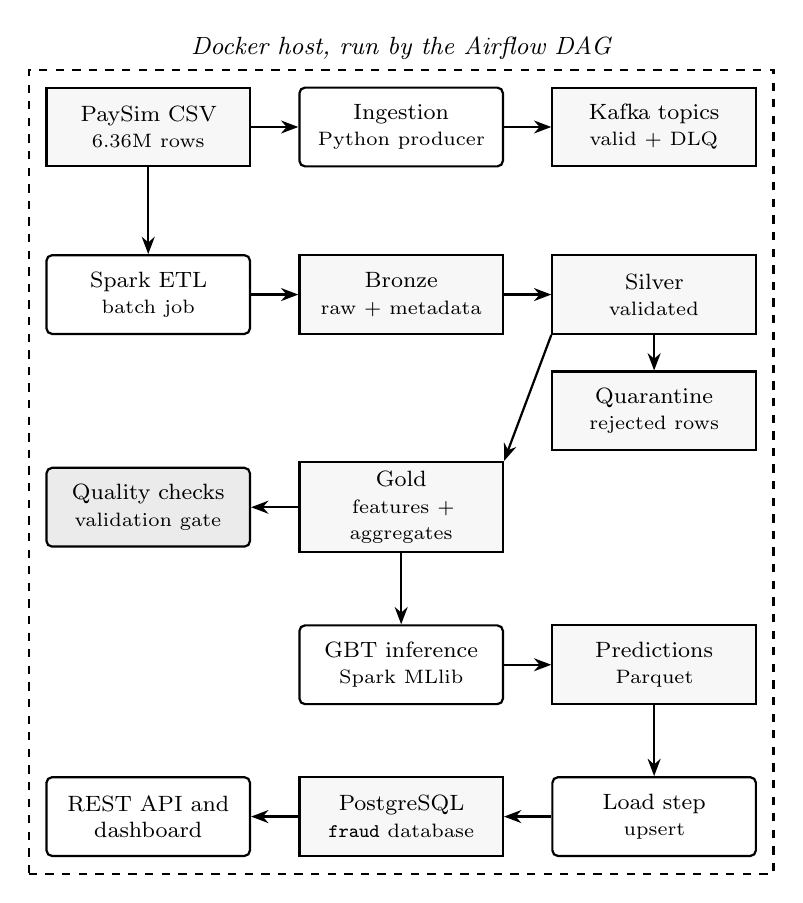
\begin{tikzpicture}[node distance=0.55cm and 0.6cm]
\node[store] (csv) {PaySim CSV\\\scriptsize 6.36M rows};
\node[proc, right=of csv] (ing) {Ingestion\\\scriptsize Python producer};
\node[store, right=of ing] (kafka) {Kafka topics\\\scriptsize valid + DLQ};

\node[proc, below=1.1cm of csv] (etl) {Spark ETL\\\scriptsize batch job};
\node[store, right=of etl] (bronze) {Bronze\\\scriptsize raw + metadata};
\node[store, right=of bronze] (silver) {Silver\\\scriptsize validated};
\node[store, below=0.45cm of silver] (quar) {Quarantine\\\scriptsize rejected rows};
\node[store, below=1.6cm of bronze] (gold) {Gold\\\scriptsize features + aggregates};

\node[tproc, left=of gold] (qc) {Quality checks\\\scriptsize validation gate};
\node[proc, below=0.9cm of gold] (ml) {GBT inference\\\scriptsize Spark MLlib};
\node[store, right=of ml] (pred) {Predictions\\\scriptsize Parquet};
\node[proc, below=0.9cm of pred] (load) {Load step\\\scriptsize upsert};
\node[store, left=of load] (pg) {PostgreSQL\\\scriptsize \code{fraud} database};
\node[proc, left=of pg] (api) {REST API and\\dashboard};

\draw[arr] (csv) -- (ing);
\draw[arr] (ing) -- (kafka);
\draw[arr] (csv) -- (etl);
\draw[arr] (etl) -- (bronze);
\draw[arr] (bronze) -- (silver);
\draw[arr] (silver) -- (quar);
\draw[arr] (silver.south west) -- (gold.north east);
\draw[arr] (gold) -- (qc);
\draw[arr] (gold) -- (ml);
\draw[arr] (ml) -- (pred);
\draw[arr] (pred) -- (load);
\draw[arr] (load) -- (pg);
\draw[arr] (pg) -- (api);

\node[draw, dashed, thick, inner sep=6pt, fit=(ing)(etl)(qc)(ml)(load)(kafka)(quar)(api),
      label={[font=\small\itshape]above:Docker host, run by the Airflow DAG}] {};
\end{tikzpicture}
\caption{System architecture. Shaded boxes are data stores; white boxes are processing stages}
\label{fig:architecture}
\end{figure}

\paragraph{Medallion layers.}
\begin{itemize}
  \item \textbf{Bronze} (\code{data/bronze/transactions}) holds every source record
        as it was received, with a batch identifier, an ingestion timestamp, the
        source system and a SHA-256 hash of the record added. It is partitioned by
        \code{step}.
  \item \textbf{Silver} (\code{data/silver/transactions}) holds properly typed
        records that pass seven business rules, with duplicates removed on a
        composite business key. Rejected records go to
        \code{data/quarantine/transactions}, along with the reason and the time
        they were rejected.
  \item \textbf{Gold} (\code{data/gold}) holds \code{enriched\_transactions}, which
        adds a stable \code{transaction\_id} and ten engineered features, plus two
        summary tables, \code{customer\_aggregates} and \code{hourly\_aggregates}.
\end{itemize}

\subsection{ETL and ELT in the Platform}
Different parts of the platform follow different patterns, and we chose each one
for a reason (Figure~\ref{fig:patterns}, Table~\ref{tab:patterns}).

\paragraph{Ingestion into Kafka.} The producer reads the CSV in chunks and sends
each record to Kafka without changing its content. The only thing that happens
before loading is validation, which decides whether a record goes to the main
topic or to the dead-letter topic.

\paragraph{ELT in the lakehouse.} The ETL lands the raw records in Bronze first,
and only then derives Silver and Gold from them with Spark. Because the raw copy
is kept, we can change a rule or a feature later and rebuild Silver and Gold
without going back to the source.

\paragraph{Scoring and serving.} Inference turns Gold into predictions. Loading
those predictions into PostgreSQL is a plain extract and load, with nothing more
than a type mapping.

\begin{figure}[H]
\centering
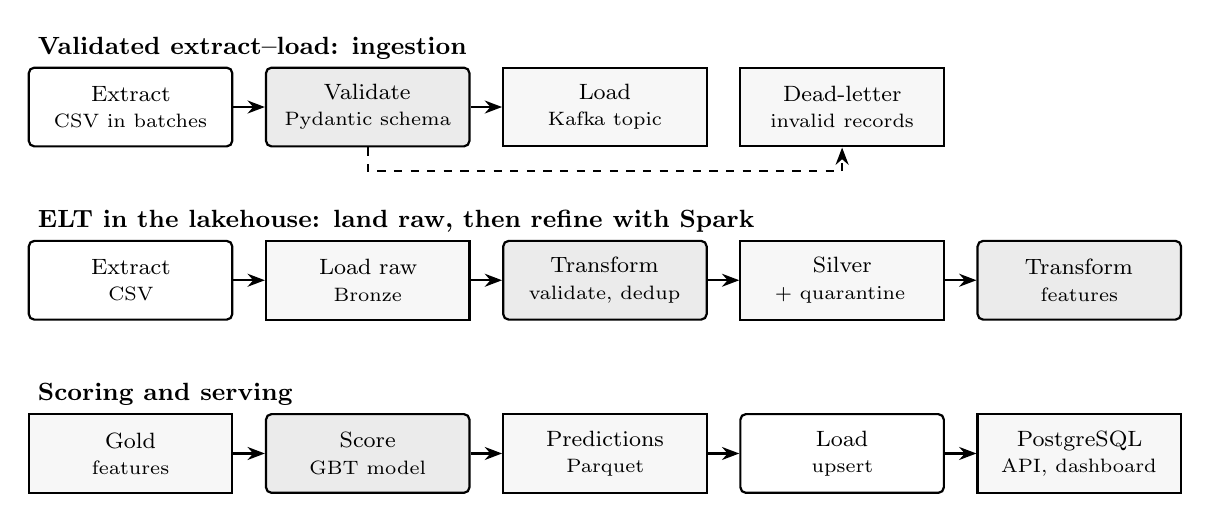
\begin{tikzpicture}[node distance=0.4cm]
\node[font=\small\bfseries, anchor=west] at (-1.3,0.75) {Validated extract--load: ingestion};
\node[proc] (a1) at (0,0) {Extract\\\scriptsize CSV in batches};
\node[tproc, right=of a1] (a2) {Validate\\\scriptsize Pydantic schema};
\node[store, right=of a2] (a3) {Load\\\scriptsize Kafka topic};
\node[store, right=of a3] (a4) {Dead-letter\\\scriptsize invalid records};
\draw[arr] (a1) -- (a2);
\draw[arr] (a2) -- (a3);
\draw[darr] (a2.south) -- ++(0,-0.3) -| (a4.south);

\node[font=\small\bfseries, anchor=west] at (-1.3,-1.45) {ELT in the lakehouse: land raw, then refine with Spark};
\node[proc] (b1) at (0,-2.2) {Extract\\\scriptsize CSV};
\node[store, right=of b1] (b2) {Load raw\\\scriptsize Bronze};
\node[tproc, right=of b2] (b3) {Transform\\\scriptsize validate, dedup};
\node[store, right=of b3] (b4) {Silver\\\scriptsize + quarantine};
\node[tproc, right=of b4] (b5) {Transform\\\scriptsize features};
\draw[arr] (b1) -- (b2);
\draw[arr] (b2) -- (b3);
\draw[arr] (b3) -- (b4);
\draw[arr] (b4) -- (b5);

\node[font=\small\bfseries, anchor=west] at (-1.3,-3.65) {Scoring and serving};
\node[store] (c1) at (0,-4.4) {Gold\\\scriptsize features};
\node[tproc, right=of c1] (c2) {Score\\\scriptsize GBT model};
\node[store, right=of c2] (c3) {Predictions\\\scriptsize Parquet};
\node[proc, right=of c3] (c4) {Load\\\scriptsize upsert};
\node[store, right=of c4] (c5) {PostgreSQL\\\scriptsize API, dashboard};
\draw[arr] (c1) -- (c2);
\draw[arr] (c2) -- (c3);
\draw[arr] (c3) -- (c4);
\draw[arr] (c4) -- (c5);
\end{tikzpicture}
\caption{Where each pattern is used. Shaded boxes are transformation steps}
\label{fig:patterns}
\end{figure}

\begin{table}[H]
\centering
\caption{ETL and ELT steps in the platform}
\label{tab:patterns}
\begin{tabularx}{\linewidth}{lllL}
\toprule
Pipeline & Pattern & Where it transforms & Why \\
\midrule
\code{run\_ingestion.py} & EL + validation & Pydantic, per record & Invalid records must not enter the main topic \\
\code{run\_lakehouse\_etl.py} & ELT & Spark, after Bronze & Raw copy kept; layers rebuildable \\
\code{predict\_fraud.py} & ETL & Spark MLlib & Scores must match the saved pipeline \\
\code{load\_predictions\_to\_postgres.py} & EL & None beyond type mapping & Rows are already final \\
\bottomrule
\end{tabularx}
\end{table}

\subsection{Event Ingestion with Apache Kafka}

\subsubsection{Topics and Keys}
Kafka runs as a single broker in KRaft mode, so ZooKeeper is not needed. The two
topics are listed in Table~\ref{tab:topics}. Messages are keyed by the sender's
account, \code{nameOrig}, so every transaction from one account goes to the same
partition and keeps its order.

\begin{table}[H]
\centering
\caption{Kafka topic contracts}
\label{tab:topics}
\begin{tabularx}{\linewidth}{lLl}
\toprule
Topic & Content & Producer $\rightarrow$ consumer \\
\midrule
\code{financial-transactions} & Valid transactions as JSON, key \code{nameOrig} & producer $\rightarrow$ streaming ETL \\
\code{financial-transactions-dlq} & Invalid records with error message and row number & producer $\rightarrow$ operators \\
\bottomrule
\end{tabularx}
\end{table}

\subsubsection{Schema as Contract}
Before anything is published, each row is checked against a Pydantic model. The
model enforces the column types, the five allowed transaction types, non-negative
amounts and balances, a fraud label of 0 or 1 and the format of the account IDs,
and it also accepts a few alternative spellings of the column names. A row that
fails is wrapped together with the error message and its row number and sent to
the dead-letter topic, so nothing disappears without a trace.

\subsubsection{Producer Guarantees}
The producer reads the 470~MB file in batches of 5,000 rows, so its memory use
stays flat no matter how large the file is. It publishes with \code{acks=all} and
three retries, which means a record only counts as delivered once the broker has
fully stored it, and it flushes any remaining messages at the end of the run.
There is also an optional rate limiter that replays the file at a fixed number of
events per second to imitate a live feed, and a dry-run mode that validates the
file without needing a broker. Every setting can be changed through an
environment variable or a command-line flag.

\subsection{Lakehouse Processing with Apache Spark}

\subsubsection{Bronze: Raw Archive}
The batch ETL reads the source file and writes it to Bronze as Snappy-compressed
Parquet, partitioned by \code{step}, with four audit columns added. One of them is
a SHA-256 hash of the whole record, which makes it possible to spot duplicate
deliveries later on.

\subsubsection{Silver: Validation, Quarantine and De-duplication}
Silver reads from Bronze, casts each column to its proper type and applies seven
rules. The step has to be present and at least 1, the type has to be one of the
five known values, the amount has to be present and not negative, both account
IDs have to be present and well formed, and all four balances have to be present
and not negative. Records that break a rule are written to the quarantine table
together with the first rule they broke and a timestamp. The rest are
de-duplicated on a business key made up of \code{step}, \code{type},
\code{amount}, \code{nameOrig}, \code{nameDest}, \code{oldbalanceOrg} and
\code{newbalanceOrig}.

\subsubsection{Gold: Features and Aggregates}
Gold adds a \code{transaction\_id}, which is a SHA-256 hash of the business key
and therefore stays the same from one run to the next, along with the features in
Table~\ref{tab:features}. It also builds per-customer and per-hour summary
tables. The \code{isFraud} and \code{isFlaggedFraud} labels are carried through,
but only so the model can be evaluated; they are never used as inputs.

\begin{table}[H]
\centering
\caption{Engineered features in the Gold layer}
\label{tab:features}
\begin{tabularx}{\linewidth}{lL}
\toprule
Feature & Definition \\
\midrule
\code{orig\_balance\_error} & $\text{newbalanceOrig} + \text{amount} - \text{oldbalanceOrg}$ \\
\code{dest\_balance\_error} & $\text{oldbalanceDest} + \text{amount} - \text{newbalanceDest}$ \\
\code{is\_high\_risk\_type} & 1 if the type is TRANSFER or CASH\_OUT \\
\code{is\_merchant\_dest} & 1 if the receiver is a merchant (\code{M} prefix) \\
\code{is\_customer\_dest} & 1 if the receiver is a customer (\code{C} prefix) \\
\code{orig\_zero\_balance\_flag} & 1 if the sender's balance before the transaction is zero \\
\code{dest\_zero\_balance\_flag} & 1 if the receiver's balance is zero before and after \\
\code{is\_orig\_fully\_emptied} & 1 if a positive sender balance is reduced to zero \\
\code{amount\_to\_orig\_balance\_ratio} & $\text{amount} / (\text{oldbalanceOrg} + 1)$ when the balance is positive \\
\code{is\_large\_transaction} & 1 if the amount is at least 200,000 \\
\bottomrule
\end{tabularx}
\end{table}

\subsection{Fraud Detection Model}

\subsubsection{Leakage-Aware Feature Selection}
We compared three sets of features. The full set includes the balances
\emph{after} the transaction and the balance-error features worked out from
them. These are very predictive in PaySim, but a real system has to make its
decision before the payment goes through, when those values do not exist yet, so
a model trained on them would look far better than it really is. The model we
deployed uses the deployment-safe set shown in Listing~\ref{lst:modelconfig}: ten
numeric features that are available at the moment a payment is scored, plus the
transaction type, one-hot encoded.

\begin{lstlisting}[caption={Configuration of the deployed model (\code{models/member3/model\_config.json})},label={lst:modelconfig}]
{ "model_type": "GBTClassifier",
  "threshold": 0.4,
  "features": ["amount", "oldbalanceOrg", "oldbalanceDest",
               "is_high_risk_type", "is_merchant_dest", "is_customer_dest",
               "orig_zero_balance_flag", "amount_to_orig_balance_ratio",
               "is_large_transaction", "step"],
  "categorical_features": ["type"],
  "label": "isFraud",
  "test_precision": 0.7728, "test_recall": 0.7261, "test_f1": 0.7487 }
\end{lstlisting}

\subsubsection{Training Protocol}
We split Gold 80/20 into training and test sets using seed 42, then split the
training part 80/20 again (seed 123) into a set for fitting models and a
validation set that was used only to choose the threshold. That way the test set
played no part in any modelling decision. We started from a logistic regression
baseline and then tried random forests (20 trees, depth 8) and gradient-boosted
trees (20 iterations, depth 5) on each of the feature sets.

\subsubsection{Threshold Tuning}
With only 0.13\% positives, there is no reason to assume that the default
threshold of 0.5 is the right one. We scored the validation set with the
gradient-boosted model at thresholds of 0.1, 0.2, 0.3, 0.4 and 0.5 and chose 0.4,
which gave the best balance between precision and recall.

\subsubsection{Inference Contract}
The inference script reads Gold, rebuilds the deployment-safe features, applies
the saved preprocessing pipeline and model, and writes \code{transaction\_id},
\code{type}, \code{amount}, \code{step}, \code{fraud\_probability},
\code{fraud\_prediction} and \code{model\_threshold} to
\code{data/gold/fraud\_predictions}. These seven columns are the agreed contract
with the serving layer.

\subsection{Batch Orchestration with Apache Airflow}

An Airflow DAG describes which tasks have to run and in what order. The scheduler
decides when, creates a run for each interval and retries tasks that fail. For
this to be safe, every task has to be idempotent, and no task should start if the
one before it has failed.

\subsubsection{DAG Inventory}
A single DAG, \code{fraud\_detection\_pipeline}, runs the whole chain every six
hours (\code{0 */6 * * *}). Its seven tasks are listed in Table~\ref{tab:dag} in
the order in which they run.

\begin{table}[H]
\centering
\caption{Tasks of the \code{fraud\_detection\_pipeline} DAG}
\label{tab:dag}
\begin{tabularx}{\linewidth}{clL}
\toprule
\# & Task & Action and output \\
\midrule
1 & \code{member1\_ingestion} & Publish transactions to Kafka (capped at 100,000 per run) \\
2 & \code{member2\_etl} & Batch ETL: CSV $\rightarrow$ Bronze $\rightarrow$ Silver $\rightarrow$ Gold, overwriting each layer \\
3 & \code{member4\_quality\_checks} & Validation gate: each layer exists, is readable Parquet and is not empty \\
4 & \code{member3\_fraud\_detection} & Score Gold with the saved model; write predictions \\
5 & \code{member5\_load\_predictions} & Upsert predictions into PostgreSQL and log the load \\
6 & \code{pipeline\_health\_check} & Confirm that every layer and the predictions exist \\
7 & \code{pipeline\_success} & Record successful completion \\
\bottomrule
\end{tabularx}
\end{table}

\subsubsection{Anatomy of a Task}
Each task runs one of the stage scripts as a subprocess from the project root, so
a task in Airflow and a manual run execute exactly the same code. If the script
returns a non-zero exit code, the task fails and Airflow does not start anything
downstream (Figure~\ref{fig:dag}). The DAG finds the project root by searching
upwards for the \code{scripts} folder, which lets the same file work both in the
repository and inside the container. An earlier version counted a fixed number of
parent folders instead, and it broke as soon as it ran in Docker.

\begin{lstlisting}[caption={Task order in the DAG},label={lst:deps}]
ingest_task >> etl_task >> quality_task >> inference_task \
    >> load_task >> health_check_task >> success_task
\end{lstlisting}

\begin{figure}[H]
\centering
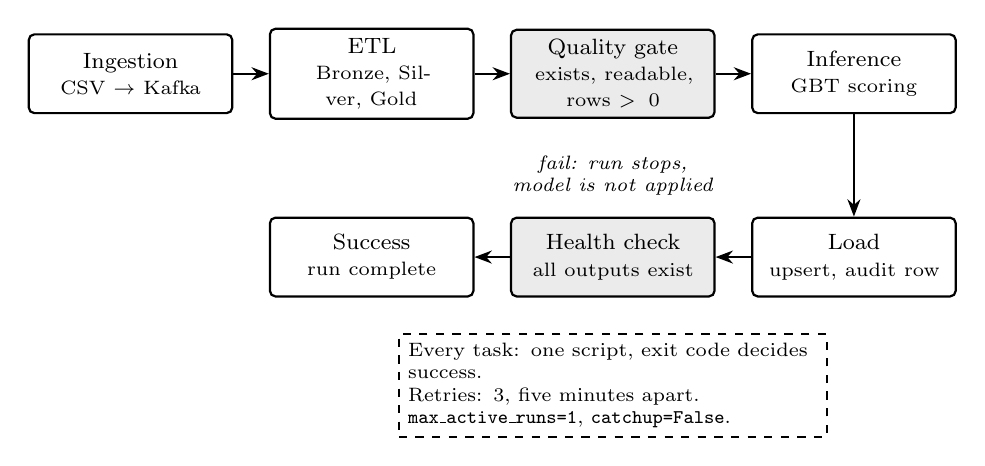
\begin{tikzpicture}[node distance=0.45cm and 0.45cm]
\node[proc] (t1) {Ingestion\\\scriptsize CSV $\rightarrow$ Kafka};
\node[proc, right=of t1] (t2) {ETL\\\scriptsize Bronze, Silver, Gold};
\node[tproc, right=of t2] (t3) {Quality gate\\\scriptsize exists, readable, rows $>0$};
\node[proc, right=of t3] (t4) {Inference\\\scriptsize GBT scoring};
\node[proc, below=1.3cm of t4] (t5) {Load\\\scriptsize upsert, audit row};
\node[tproc, left=of t5] (t6) {Health check\\\scriptsize all outputs exist};
\node[proc, left=of t6] (t7) {Success\\\scriptsize run complete};
\draw[arr] (t1) -- (t2);
\draw[arr] (t2) -- (t3);
\draw[arr] (t3) -- (t4);
\draw[arr] (t4) -- (t5);
\draw[arr] (t5) -- (t6);
\draw[arr] (t6) -- (t7);
\node[note, below=0.35cm of t3] {fail: run stops,\\model is not applied};
\node[draw, thick, dashed, align=left, font=\scriptsize, text width=5.2cm, below=0.45cm of t6]
  {Every task: one script, exit code decides success.\\
   Retries: 3, five minutes apart.\\
   \code{max\_active\_runs=1}, \code{catchup=False}.};
\end{tikzpicture}
\caption{Anatomy of the DAG: stage tasks, validation gates and shared reliability settings}
\label{fig:dag}
\end{figure}

\subsubsection{Validation Gates}
The quality task reads each layer with Spark and fails the run if a layer is
missing, cannot be read as Parquet or has no rows. Since inference depends on this
task, the model never runs on an empty or broken Gold table, and a half-finished
ETL cannot quietly produce zero alerts that look like a clean run. At the very
end, the health check confirms that every layer and the prediction output exist.

\subsubsection{Reliability Settings}
\begin{itemize}
  \item \textbf{Retries.} Every task is retried up to three times, five minutes
        apart. This covers short outages, such as Kafka still starting up when
        the run begins.
  \item \textbf{One run at a time.} With \code{max\_active\_runs=1}, two runs can
        never write to the same layers at once.
  \item \textbf{No backlog.} With \code{catchup=False}, a DAG that has been paused
        for a while does not try to make up every missed interval; it simply runs
        once for the latest one.
  \item \textbf{Safe re-runs.} The ETL overwrites Bronze, Silver and Gold, and the
        load is an upsert, so a retry gives the same result as the first attempt.
  \item \textbf{Failure notices.} A failed task can send an e-mail once an SMTP
        server is configured; either way, failures are visible in the Airflow UI.
\end{itemize}

\subsection{Serving Layer}

\subsubsection{PostgreSQL Store}
We load the predictions into a separate database called \code{fraud}, on the same
PostgreSQL server that holds Airflow's metadata, so that the two do not mix. The
\code{fraud\_predictions} table uses \code{transaction\_id} as its primary key and
checks that the probability lies between 0 and 1 and that the prediction is 0 or
1. An index on \code{fraud\_probability} keeps the alert query fast. The whole
load happens in one transaction using the upsert in Listing~\ref{lst:upsert}, so
re-running it updates existing rows rather than duplicating them, and if it fails
the previous data is left as it was. Every load is also logged in
\code{pipeline\_runs} with its status, row count, any error message and its
timing.

\begin{lstlisting}[language=SQL,caption={Idempotent load into the serving table (abridged)},label={lst:upsert}]
INSERT INTO fraud_predictions (transaction_id, type, amount, step,
       fraud_probability, fraud_prediction, model_threshold) VALUES %s
ON CONFLICT (transaction_id) DO UPDATE SET
       fraud_probability = EXCLUDED.fraud_probability,
       fraud_prediction  = EXCLUDED.fraud_prediction,
       ...,
       loaded_at = now()
\end{lstlisting}

\subsubsection{REST API}
A FastAPI service exposes the endpoints in Table~\ref{tab:api}. If someone calls it
before anything has been loaded, it replies with HTTP 503 and a clear message
instead of failing with an internal error, and interactive documentation is
generated automatically at \code{/docs}.

\begin{table}[H]
\centering
\caption{REST API endpoints}
\label{tab:api}
\begin{tabularx}{\linewidth}{lL}
\toprule
Endpoint & Returns \\
\midrule
\code{GET /health} & Service and database status \\
\code{GET /alerts} & Flagged transactions, highest probability first; optional \code{min\_probability} and \code{limit} \\
\code{GET /transactions/\{id\}} & One scored transaction, or 404 \\
\code{GET /stats} & Totals, flagged counts by type, recent loads and model metrics \\
\code{GET /} & The analyst dashboard \\
\bottomrule
\end{tabularx}
\end{table}

\subsubsection{Analyst Dashboard}
The same application serves a single web page for analysts who would rather not
work with an API directly. It shows whether the service is up, each stage of the
pipeline and how the last run went, and the headline numbers: transactions
scored, transactions flagged and how well the model performs. Below that are a
chart of alerts by transaction type, the list of flagged transactions with a
slider to change the probability cut-off, and a lookup that shows the score and
verdict for any single transaction.

\subsection{Delivering the Platform}

\subsubsection{Containerised Deployment}
All the services are defined in one \code{docker-compose.yml}
(Table~\ref{tab:services}). The Airflow image is based on
\code{apache/airflow:2.7.2-python3.11}, with a Java~17 runtime added for Spark and
the project's Python libraries installed on top. The source code, scripts, model,
dataset and data folders are mounted into the containers, so a code change takes
effect without rebuilding anything and the lakehouse files stay on the host.

\begin{table}[H]
\centering
\caption{Containerised services}
\label{tab:services}
\begin{tabularx}{\linewidth}{lLl}
\toprule
Service & Purpose & Port \\
\midrule
\code{kafka} & Kafka broker in KRaft mode & 9092 \\
\code{kafka-ui} & Web viewer for topics and messages & 8080 \\
\code{postgres} & Airflow metadata and the \code{fraud} serving database & 5432 \\
\code{airflow-init} & One-off database set-up and admin user & -- \\
\code{airflow-webserver} & Airflow user interface & 8081 \\
\code{airflow-scheduler} & Schedules and runs the DAG tasks & -- \\
\code{api} & FastAPI service and dashboard & 8000 \\
\bottomrule
\end{tabularx}
\end{table}

\subsubsection{Platform Practices}
\begin{itemize}
  \item \textbf{One command to start.} Running \code{docker compose up -d --build}
        brings up every service. Airflow creates its own database and admin user
        the first time, and the load step creates the serving database and its
        tables if they are missing.
  \item \textbf{Pinned versions.} Spark is pinned to 4.2.0, the version the model
        was saved with, and libraries that clash with Airflow~2.7.2 are held to
        compatible versions, so the image builds the same way every time.
  \item \textbf{Same code everywhere.} Each stage is a script that the DAG calls
        and that anyone can also run by hand, which makes problems easy to
        reproduce.
  \item \textbf{Documentation.} Each component has its own guide in \code{docs/},
        and there is a separate guide for running the demonstration.
\end{itemize}

\subsubsection{Data Products and Access Formats}
Every layer is stored in an open format that can be read with standard tools
(Table~\ref{tab:products}), so nobody needs a special client to use the data.

\begin{table}[H]
\centering
\caption{Data products, formats and how to access them}
\label{tab:products}
\begin{tabularx}{\linewidth}{lLlL}
\toprule
Layer & Product & Format & Access \\
\midrule
Stream & \code{financial-transactions}, \code{financial-transactions-dlq} & JSON & Any Kafka consumer; Kafka UI \\
Bronze & \code{data/bronze/transactions} & Parquet & Spark, PyArrow, pandas \\
Silver & \code{data/silver/transactions}, \code{data/quarantine/transactions} & Parquet & Spark, PyArrow, pandas \\
Gold & \code{enriched\_transactions}, \code{customer\_aggregates}, \code{hourly\_aggregates} & Parquet & Spark, PyArrow, pandas \\
Predictions & \code{data/gold/fraud\_predictions} & Parquet & Spark, PyArrow \\
Serving & \code{fraud\_predictions}, \code{pipeline\_runs} & PostgreSQL & SQL (psql), REST API, dashboard \\
\bottomrule
\end{tabularx}
\end{table}

% ===========================================================================
\section{Results and Evaluation}
% ===========================================================================

\subsection{Pipeline Operation}
We ran the DAG on the full PaySim file inside the Docker stack. All seven tasks
succeeded and the run took about 24 minutes (Table~\ref{tab:run}). Every layer
held exactly 6,362,620 rows, so no record was lost, duplicated or quarantined
between Bronze and Gold, which is what we expected from a clean synthetic source.
Loading all the predictions into PostgreSQL took 3 minutes 29 seconds, and alert
queries that use the probability index come back in milliseconds. Getting to this
point took several attempts; the problems we hit along the way are described in
Section~\ref{sec:issues}. Figure~\ref{fig:airflow} shows a completed run in
Airflow, and Figure~\ref{fig:dashboard} shows the dashboard afterwards.

\begin{table}[H]
\centering
\caption{Full-dataset run}
\label{tab:run}
\begin{tabular}{lr}
\toprule
Measure & Value \\
\midrule
Rows in Bronze, Silver and Gold & 6,362,620 each \\
Rows quarantined & 0 \\
Transactions flagged at threshold 0.4 & 7,598 \\
Rows loaded into PostgreSQL & 6,362,620 \\
PostgreSQL load time & 3 min 29 s \\
End-to-end DAG duration & about 24 min \\
Highest fraud probability served & 0.997 \\
\bottomrule
\end{tabular}
\end{table}

\begin{figure}[H]
\centering
\screenshot{figures/airflow_graph.png}{5.5cm}
\caption{Airflow graph view of a successful run of \code{fraud\_detection\_pipeline}}
\label{fig:airflow}
\end{figure}

\begin{figure}[H]
\centering
\screenshot{figures/dashboard.png}{7cm}
\caption{Analyst dashboard after the full-dataset run}
\label{fig:dashboard}
\end{figure}

\subsection{Data Quality}
We check data quality in three places. At ingestion, every record is validated
and failures go to the dead-letter topic. In Silver, seven rules send failing
records to quarantine with a reason, and duplicates are removed on the business
key. Between Gold and the model, the validation gate stops the run if any layer is
missing, unreadable or empty. On the full dataset everything passed and nothing
was quarantined. Clean data does not really put these rules to the test, so we
also rely on the automated tests. Their synthetic input contains three
deliberately bad records (a negative amount, an unknown transaction type and a
negative balance), and the tests confirm that exactly these three end up in
quarantine with the right reasons and that duplicate rows are reduced to one.

\subsection{Model Performance}
Table~\ref{tab:confusion} shows the confusion matrix for the deployed model over
the full dataset, and Table~\ref{tab:metrics} the metrics that follow from it.
The full dataset also contains the rows the model was trained on, so the fair
estimate is the held-out test result recorded during training, which we report
alongside.

\begin{table}[H]
\centering
\caption{Confusion matrix on the full dataset at threshold 0.4}
\label{tab:confusion}
\begin{tabular}{lrr}
\toprule
 & Predicted fraud & Predicted genuine \\
\midrule
Actual fraud   & 5,938 (TP) & 2,275 (FN) \\
Actual genuine & 1,660 (FP) & 6,352,747 (TN) \\
\bottomrule
\end{tabular}
\end{table}

\begin{table}[H]
\centering
\caption{Classification metrics}
\label{tab:metrics}
\begin{tabular}{lccc}
\toprule
Evaluation set & Precision & Recall & F1 \\
\midrule
Held-out test split (unbiased) & 0.773 & 0.726 & 0.749 \\
Full dataset (includes training rows) & 0.782 & 0.723 & 0.751 \\
\bottomrule
\end{tabular}
\end{table}

The metrics are defined as
\begin{equation}
\text{Precision} = \frac{TP}{TP+FP}, \qquad
\text{Recall} = \frac{TP}{TP+FN}, \qquad
F_1 = \frac{2\cdot\text{Precision}\cdot\text{Recall}}{\text{Precision}+\text{Recall}}.
\end{equation}
Over the full dataset, 5,938 of the 7,598 alerts ($0.782$) were real fraud, and
5,938 of the 8,213 fraud cases ($0.723$) were caught. These figures are very close
to the test results, which suggests that the model is not overfitting.

In practical terms, about four out of every five alerts are genuine fraud, so an
analyst's time is mostly well spent, and roughly 72\% of fraud is caught without
anyone having to look for it. Across the 31 simulated days the model raised 7,598
alerts, or about 245 a day, which a small team could realistically review. The
2,275 frauds it missed are the price of the threshold we chose: lowering it would
catch more fraud but would also flag more genuine customers. Almost all the alerts
are TRANSFER or CASH\_OUT transactions, which is where the fraud actually is. The
handful on other types are false positives that a simple business rule could
filter out.

\subsection{Testing}
The repository has 50 automated tests (Table~\ref{tab:tests}). The lakehouse and
ETL tests run on a local Spark session using a small synthetic file with valid,
fraudulent and invalid rows, so we know in advance exactly what every count should
be. The serving tests use a separate \code{fraud\_test} database and skip
themselves if PostgreSQL is not running. Before trying the full dataset, we also
ran the complete DAG in Docker on the 12-row sample file, to make sure all seven
tasks succeeded and the API returned the flagged transaction.

\begin{table}[H]
\centering
\caption{Automated test suites}
\label{tab:tests}
\begin{tabularx}{\linewidth}{lrL}
\toprule
Suite & Tests & Scope \\
\midrule
\code{test\_models.py} & 10 & Validation and rejection rules, alias normalisation, Kafka serialisation \\
\code{test\_reader.py} & 6 & Incremental reading, batching, record limits, missing files \\
\code{test\_producer.py} & 4 & Publishing and DLQ in dry-run mode, mocked Kafka client, rate limiter \\
\code{test\_pipeline.py} & 3 & Ingestion on synthetic data, record limits, graceful stop \\
\code{test\_lakehouse.py} & 10 & Casting, Silver rules, de-duplication, identifiers, features, aggregates, layer I/O \\
\code{test\_etl.py} & 6 & End-to-end ETL, repeated runs, limits, empty and JSON input, bad formats \\
\code{test\_serving.py} & 11 & Upsert behaviour, failure logging, API responses and errors \\
\midrule
Total & 50 & \\
\bottomrule
\end{tabularx}
\end{table}

\subsection{Guarantees Verified}
At every hand-over between stages there is a key or a rule that makes repeating
the step harmless (Figure~\ref{fig:idempotency}). This is what lets us rely on
retries: Airflow may run a task more than once, but each transaction still ends
up in the results exactly once.

\begin{figure}[H]
\centering
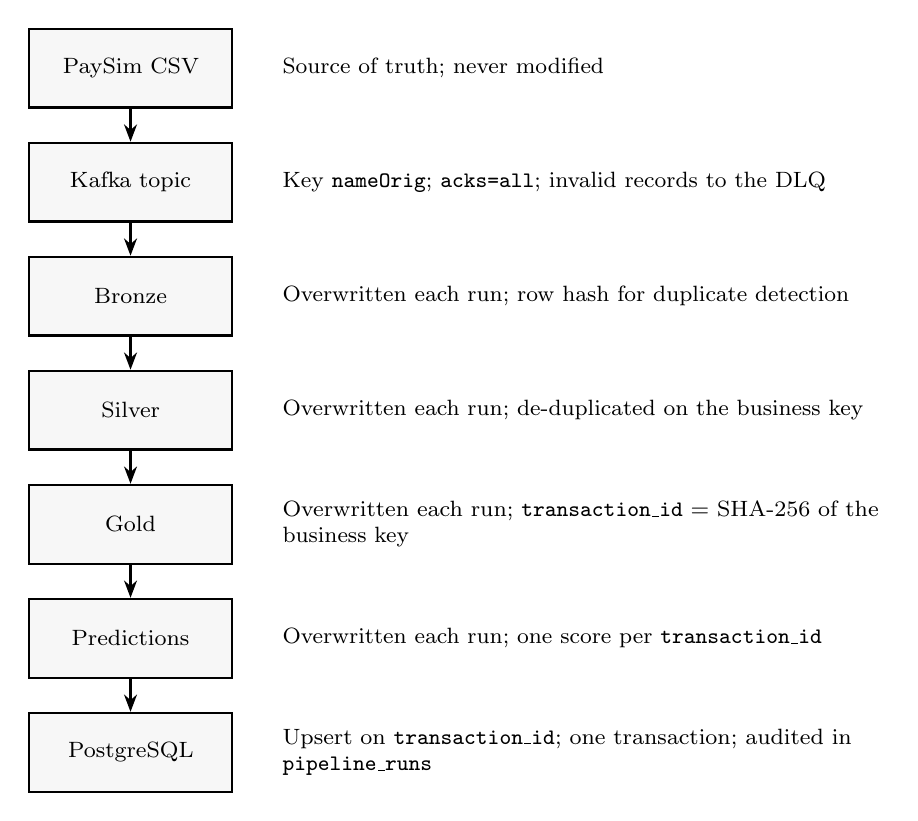
\begin{tikzpicture}[node distance=0.42cm]
\tikzset{key/.style={font=\footnotesize, align=left, text width=7.6cm, anchor=west}}
\node[store] (k1) {PaySim CSV};
\node[store, below=of k1] (k2) {Kafka topic};
\node[store, below=of k2] (k3) {Bronze};
\node[store, below=of k3] (k4) {Silver};
\node[store, below=of k4] (k5) {Gold};
\node[store, below=of k5] (k6) {Predictions};
\node[store, below=of k6] (k7) {PostgreSQL};
\foreach \a/\b in {k1/k2, k2/k3, k3/k4, k4/k5, k5/k6, k6/k7} \draw[arr] (\a) -- (\b);
\node[key] at ($(k1.east)+(0.5,0)$) {Source of truth; never modified};
\node[key] at ($(k2.east)+(0.5,0)$) {Key \code{nameOrig}; \code{acks=all}; invalid records to the DLQ};
\node[key] at ($(k3.east)+(0.5,0)$) {Overwritten each run; row hash for duplicate detection};
\node[key] at ($(k4.east)+(0.5,0)$) {Overwritten each run; de-duplicated on the business key};
\node[key] at ($(k5.east)+(0.5,0)$) {Overwritten each run; \code{transaction\_id} = SHA-256 of the business key};
\node[key] at ($(k6.east)+(0.5,0)$) {Overwritten each run; one score per \code{transaction\_id}};
\node[key] at ($(k7.east)+(0.5,0)$) {Upsert on \code{transaction\_id}; one transaction; audited in \code{pipeline\_runs}};
\end{tikzpicture}
\caption{End-to-end idempotency: the key or rule that makes each hop safe to repeat}
\label{fig:idempotency}
\end{figure}

Table~\ref{tab:failures} lists the failure cases we designed for and what happens
in each one.

\begin{table}[H]
\centering
\caption{Failure scenarios and how the platform handles them}
\label{tab:failures}
\begin{tabularx}{\linewidth}{lL}
\toprule
Scenario & Mechanism and outcome \\
\midrule
Broker or service briefly unavailable & Airflow retries the task up to three times, five minutes apart \\
Malformed or out-of-rule source record & Dead-letter topic at ingestion; quarantine with a reason in Silver \\
Duplicate source rows & Removed in Silver on the business key \\
Task re-run after a partial write & Layers are overwritten and the load is an upsert: no duplicates \\
ETL produces a missing or empty layer & Validation gate fails; the model is not applied \\
Load fails part-way & Single transaction rolls back; old data stays; run marked \code{failed} \\
Two runs overlap & Prevented by \code{max\_active\_runs=1} \\
API queried before any load & HTTP 503 with an explanatory message instead of an error \\
\bottomrule
\end{tabularx}
\end{table}

\subsection{Integration Issues Found and Resolved}\label{sec:issues}
Most of our problems did not come from any single component. They appeared when
everything ran together in one container environment for the first time
(Table~\ref{tab:issues}). Looking back, they are typical of a system built by
several people in parallel: each part worked on its owner's machine, but
versions, paths and file permissions did not line up once the parts were put
together.

\begin{table}[H]
\centering
\caption{Integration issues and their resolution}
\label{tab:issues}
\begin{tabularx}{\linewidth}{LL}
\toprule
Symptom & Cause and fix \\
\midrule
Saved model failed to load & Saved with Spark 4.2.0, image had 3.5; Spark pinned to 4.2.0 \\
Airflow image would not build & Base image's package repositories retired; Java copied from the Eclipse Temurin image \\
\code{import pyarrow} failed & Newest pyarrow needs NumPy 2, Airflow 2.7.2 ships NumPy 1.24; pyarrow capped below 20 \\
Every task failed with a missing script & Project root resolved to \code{/opt} in the container; now found by searching for \code{scripts} \\
ETL could not read its input & DAG passed \code{--format parquet} for a CSV; corrected \\
Spark could not write output & Host-owned files not writable by the container user; user ID made configurable \\
Batch ETL raised \code{ImportError} & Shared telemetry class removed during a merge; restored \\
Duplicate identifiers in Gold & Bronze and Silver appended on every run; switched to overwrite \\
\bottomrule
\end{tabularx}
\end{table}

\subsection{Discussion}
The most important design decision was to give each tool one job and to connect
the stages only through agreed formats: the Kafka message format, the Bronze,
Silver and Gold layouts, the prediction columns and the PostgreSQL primary key.
This made every hand-over safe to repeat, and it means any one component could be
replaced without touching the others. The platform still has some clear
limitations.
\begin{itemize}
  \item \textbf{It is batch, not real time.} Kafka ingestion runs inside the DAG,
        but the scheduled ETL reads the CSV directly, so alerts appear every six
        hours rather than as transactions arrive. There is a Spark Structured
        Streaming ETL in the code, but its Kafka connector was built for Spark 3.5
        and Scala 2.12 and does not work with the Spark 4.2.0 runtime.
  \item \textbf{The validation gate is basic.} It checks that each layer exists
        and is not empty, but it does not yet compare row counts between layers,
        check that keys are unique or confirm that the model's input features are
        present. The quarantine table is also appended to on every run, so rejects
        from earlier runs stay in it.
  \item \textbf{It runs on one machine.} The whole stack sits on a single Docker
        host, which is a single point of failure. A full run also needs about
        11~GB of memory for Docker, and with less than that the Spark stage can
        run out of memory, as we found on some of our own laptops.
  \item \textbf{The data is synthetic.} PaySim is clean and its fraud pattern is
        simple. Real data would bring noise, behaviour that changes over time and
        fraudsters who adapt to whatever the model catches.
  \item \textbf{Some operational pieces are missing.} The API has no
        authentication, failure e-mails need an SMTP server to be set up, and the
        generated lakehouse files are kept inside the repository.
\end{itemize}

% ===========================================================================
\section{Conclusion}
% ===========================================================================

We built a working fraud detection platform that ingests, cleans, scores and
serves 6.36 million transactions in about 24 minutes on a single machine, with
Airflow scheduling and monitoring every step. Kafka carries the validated records
and keeps the rejected ones in a dead-letter topic. The Spark lakehouse keeps every
raw record, sets invalid ones aside with a reason and produces the features the
model needs. The gradient-boosted model, trained without leaked information,
catches 72\% of fraud, and about four in five of its alerts are real. Finally, a
load that either fully succeeds or changes nothing puts the results behind a REST
API and a dashboard, and the whole stack starts with one Docker Compose command.

Splitting the work by pipeline stage let the five of us develop in parallel, but
the project also taught us that integration needs time of its own: most of our
hardest problems only showed up once everything ran together. The obvious next
steps are to run the streaming ETL continuously with a Kafka connector that
matches Spark 4, add stronger checks to the validation gate, monitor the model for
drift and retrain it on a schedule, and move the platform to managed cloud
services with proper authentication on the API.

% ===========================================================================
\begin{thebibliography}{99}

\bibitem[{Airflow}(2023)]{airflow}
Apache Software Foundation (2023). \emph{Apache Airflow 2.7 Documentation}.
\url{https://airflow.apache.org/docs/apache-airflow/2.7.2/}

\bibitem[Akidau et~al.(2015)]{akidau2015dataflow}
Akidau, T., Bradshaw, R., Chambers, C., et al. (2015). The Dataflow model: a
practical approach to balancing correctness, latency, and cost in massive-scale,
unbounded, out-of-order data processing. \emph{Proceedings of the VLDB
Endowment}, 8(12), 1792--1803.

\bibitem[Armbrust et~al.(2021)]{armbrust2021lakehouse}
Armbrust, M., Ghodsi, A., Xin, R., \& Zaharia, M. (2021). Lakehouse: a new
generation of open platforms that unify data warehousing and advanced analytics.
\emph{Proceedings of CIDR 2021}.

\bibitem[Breiman(2001)]{breiman2001random}
Breiman, L. (2001). Random forests. \emph{Machine Learning}, 45(1), 5--32.

\bibitem[Dal~Pozzolo et~al.(2015)]{dalpozzolo2015calibrating}
Dal Pozzolo, A., Caelen, O., Johnson, R. A., \& Bontempi, G. (2015). Calibrating
probability with undersampling for unbalanced classification. \emph{Proceedings
of the IEEE Symposium Series on Computational Intelligence}, 159--166.

\bibitem[{FastAPI}(2024)]{fastapi}
Ram\'{\i}rez, S. (2024). \emph{FastAPI Documentation}.
\url{https://fastapi.tiangolo.com/}

\bibitem[Friedman(2001)]{friedman2001greedy}
Friedman, J. H. (2001). Greedy function approximation: a gradient boosting
machine. \emph{Annals of Statistics}, 29(5), 1189--1232.

\bibitem[Kleppmann(2017)]{kleppmann2017designing}
Kleppmann, M. (2017). \emph{Designing Data-Intensive Applications}. O'Reilly Media.

\bibitem[Kreps(2014)]{kreps2014lambda}
Kreps, J. (2014). Questioning the Lambda architecture. \emph{O'Reilly Radar}.

\bibitem[Kreps et~al.(2011)]{kreps2011kafka}
Kreps, J., Narkhede, N., \& Rao, J. (2011). Kafka: a distributed messaging system
for log processing. \emph{Proceedings of the NetDB Workshop}, Athens.

\bibitem[Lopez-Rojas et~al.(2016)]{lopezrojas2016paysim}
Lopez-Rojas, E. A., Elmir, A., \& Axelsson, S. (2016). PaySim: a financial mobile
money simulator for fraud detection. \emph{Proceedings of the 28th European
Modeling and Simulation Symposium (EMSS)}, Larnaca, 249--255.

\bibitem[Marz and Warren(2015)]{marz2015bigdata}
Marz, N., \& Warren, J. (2015). \emph{Big Data: Principles and Best Practices of
Scalable Real-Time Data Systems}. Manning.

\bibitem[{Parquet}(2024)]{parquet}
Apache Software Foundation (2024). \emph{Apache Parquet Documentation}.
\url{https://parquet.apache.org/docs/}

\bibitem[{PostgreSQL}(2023)]{postgres}
PostgreSQL Global Development Group (2023). \emph{PostgreSQL 15 Documentation:
INSERT}. \url{https://www.postgresql.org/docs/15/sql-insert.html}

\bibitem[Saito and Rehmsmeier(2015)]{saito2015precision}
Saito, T., \& Rehmsmeier, M. (2015). The precision-recall plot is more informative
than the ROC plot when evaluating binary classifiers on imbalanced datasets.
\emph{PLoS ONE}, 10(3), e0118432.

\bibitem[Zaharia et~al.(2016)]{zaharia2016spark}
Zaharia, M., Xin, R. S., Wendell, P., et al. (2016). Apache Spark: a unified
engine for big data processing. \emph{Communications of the ACM}, 59(11), 56--65.

\end{thebibliography}

\end{document}
